\documentclass{article}
\usepackage{amsmath}
\usepackage{graphicx}
\usepackage[utf8]{inputenc}
%\usepackage[T1, T2A]{fontenc}
%\usepackage[english]{babel}

\DeclareMathOperator{\diag}{diag}
\DeclareMathOperator{\Arg}{Arg}

\title{A tight--binding model for $p$ electrons\\ with spin--orbit interaction}
\author{Anikin Evgeny, 128}

\begin{document}
\maketitle

In the following paper we will consider a tight--binding model for $p$ zone with spin--orbit
interaction.

Before we start, let us remind the Clebsch--Gordan coefficients for the case $l = 1$, 
$s = \frac{1}{2}$. Let $a_{j,m}$ annihilate the state with angular momentum $j$
and the projection $m$ ($j \in \{3/2, 1/2$\}), and $b_{m, s}$ --- the state with orbital
momentum projection $m$ ($j = 1$) and spin projection $s$.
\begin{equation}
	\begin{split}
		a_{\frac 32, \frac 32} &= b_{1,\frac 12}\\
		a_{\frac 32, \frac 12} &= \sqrt{\frac 13}b_{1, -\frac 12} 
		    + \sqrt{\frac 23} b_{0, \frac 12}\\
		a_{\frac 32, -\frac 12} &= \sqrt{\frac 23} b_{0, -\frac 12} +
		    	\sqrt{\frac 13}b_{-1, \frac 12} \\
		a_{\frac 32, -\frac 32} &= b_{-1,-\frac 12}\\
		a_{\frac 12, \frac 12} &= \sqrt{\frac 23} b_{1, -\frac 12} -
		    	\sqrt{\frac 13}b_{0, \frac 12} \\
		a_{\frac 12, -\frac 12} &= -\sqrt{\frac 13}b_{0, -\frac 12} 
			+ \sqrt{\frac 23} b_{-1, \frac 12}\\
	\end{split}
\end{equation}
After expressing the $b$ operators using $p_x$, $p_y$ and $p_z$, we immediately obtain
\begin{equation}
	\label{transform1}
	\begin{gathered}
		a_{\frac{3}{2}, \frac{3}{2}} = 
			\sqrt{\frac{1}{2}} \left(p_{x,\frac{1}{2}} - i p_{y,\frac{1}{2}}\right)\\
		a_{\frac{3}{2}, \frac{1}{2}} = 
			\sqrt{\frac{1}{6}} \left(p_{x,-\frac{1}{2}} - i p_{y,-\frac{1}{2}}\right) 
				+ \sqrt{\frac{2}{3}} p_{z, \frac{1}{2}}\\
		a_{\frac{3}{2}, -\frac{1}{2}} = 
			\sqrt{\frac{2}{3}} p_{z, -\frac{1}{2}}+
				\sqrt{\frac{1}{6}} \left(p_{x,\frac{1}{2}} + i p_{y,\frac{1}{2}}\right) \\
		a_{\frac{3}{2}, -\frac{3}{2}} = 
			\sqrt{\frac{1}{2}} \left(p_{x,-\frac{1}{2}} + i p_{y,-\frac{1}{2}}\right)\\
	\end{gathered}
\end{equation}
\begin{equation}
	\label{transform2}
	\begin{gathered}
		a_{\frac{1}{2}, \frac{1}{2}} = 
			\sqrt{\frac{1}{3}}\left(p_{x, -\frac{1}{2}} - ip_{y,-\frac{1}{2}}\right) - 
				\sqrt{\frac{1}{3}} p_{z,\frac{1}{2}}\\
		a_{\frac{1}{2}, -\frac{1}{2}} = 
			-\sqrt{\frac{1}{3}} p_{z,-\frac{1}{2}} + 
				\sqrt{\frac{1}{3}}\left(p_{x, \frac{1}{2}} + ip_{y,\frac{1}{2}}\right)
	\end{gathered}
\end{equation}
As \eqref{transform1}, \eqref{transform2} define a unitary transformation, $p$ can be easily
expressed via $a$.

The Hamiltonian is
\begin{multline}
	H_{\mathrm{full}} = -\Delta E_{SO} 
			a_{\frac{1}{2}, -\frac{1}{2}}^\dagger a_{\frac{1}{2}, -\frac{1}{2}}
			+\\
			+2 (t_{\parallel} \cos{p_x} + t_{\perp} \cos{p_y})
				p_{x,\frac 12}^\dagger p_{x,\frac 12}+\\
			+2(t_{\perp} \cos{p_x} + t_{\parallel} \cos{p_y})
				p_{y,\frac 12}^\dagger p_{y,\frac 12} +\\
			+2t_{3}( \cos{p_x} + \cos{p_y})
				p_{z,-\frac 12}^\dagger p_{z,-\frac 12} 
\end{multline}
It contains the atomic spin--orbit part and the part which depends on the interaction between
neighbour atoms.

After simple calculation we obtain the Hamiltonian matrix in the basis of $p$ operators:
\begin{multline}
	H = -\frac{E_{SO}}{3}
		\left(\begin{matrix}
			1 & i & -1 \\
			-i & 1 & i \\
			-1 & -i & 1
		\end{matrix} \right)
		+\\
		+\left(\begin{matrix}
			t_{\parallel} \cos{p_x} + t_{\perp} \cos{p_y} & 0 & 0 \\
			0 &  t_{\perp} \cos{p_x} + t_{\parallel} \cos{p_y} & 0 \\
			0 & 0 &  t_{3} (\cos{p_x} + \cos{p_y}) 
		\end{matrix} \right)
\end{multline}
The energy levels for the case $\Delta E_{SO} = 1$, $t_{\parallel} = 0.3$, $t_3 = t_{\perp} = 0.15$ 
are shown on the figure.
\begin{figure}[h]
	\centering
	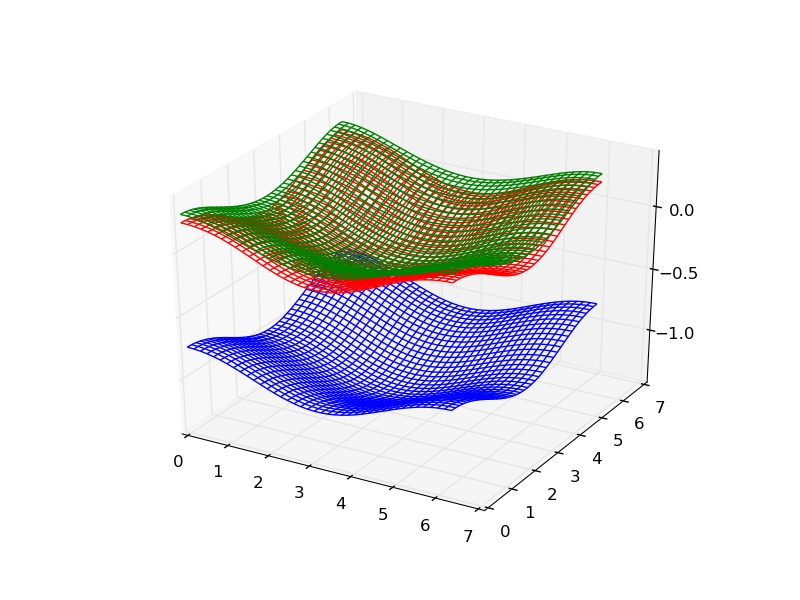
\includegraphics[width=0.6\linewidth]{tb_model/levels.jpg}
	\caption{Energy levels}
\end{figure}
\begin{figure}[h]
	\centering
	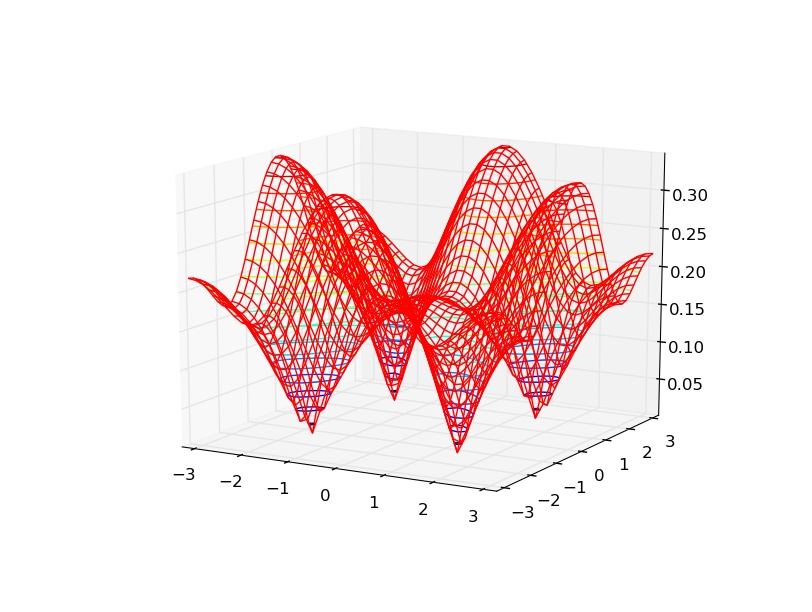
\includegraphics[width=0.6\linewidth]{tb_model/diff_levels.jpg}
	\caption{The difference of two upper energy levels}
\end{figure}

In some cases it would be (maybe) more convenient to write the Hamiltonian in the basis 
of $a$ operators. For solving that problem, the following observation would be useful.

Let $|A\rangle$ and $|B\rangle$ be the spinless states with angular momentum projections $m$ and $m'$.
Let $|A\rangle$ also be localised in $(0,0)$, and $|B(\phi)\rangle$ --- in $(r\cos{\phi}, 
r\sin{\phi}$. Then the following equation holds:
\begin{equation}
	\label{rotation_law}
	\langle A | B(\phi) \rangle = e^{-i(m-m')\phi}\langle A | B(0) \rangle
\end{equation}
That allows to write any tight--binding Hamiltonian directly in terms of $a$ states.

First Let the angle be zero, and
let the hopping integrals for the $b$ operators be described by matrix
\begin{equation}
	T_b = \left(\begin{matrix}
			t_1 & 0 & t_2 \\
			0 & t_3 & 0 \\
			t_2 & 0 & t_1
		\end{matrix}\right)
\end{equation}
The $t_i$ can be expressed via $t_{\perp}, t_{\parallel}$. 
\begin{equation}
	\begin{split}
		t_1& = \frac 12 \left(t_{\parallel} + t_{\perp}\right)\\
		t_2& = \frac 12 \left(t_{\parallel} - t_{\perp}\right)\\
	\end{split}
\end{equation}
Then for the states described by full momentum ($a$ states) we obtain
\begin{equation}
	T_x = \left(\begin{matrix}
		t_1 & \frac{1}{\sqrt{3}} t_2 & \sqrt{\frac 23} t_2 \\
		\frac{1}{\sqrt{3}}t_2 & \frac{1}{3}(t_1 + 2t_3) &\frac{\sqrt{2}}{3}(t_1 - t_3)\\
		\sqrt{\frac 23}t_2 & \frac{\sqrt{2}}{3} (t_1 - t_3) & \frac{1}{3}(2t_1 + t_3) 
		\end{matrix} \right) 
\end{equation}
For the arbitrary angle, as follows from \ref{rotation_law}, 
\begin{multline}
	T_{\phi} = \diag(e^{\frac{-3i\phi}{2}},e^{\frac{i\phi}{2}},e^{\frac{i\phi}{2}})
				\times T_x 
				\times \diag(e^{\frac{3i\phi}{2}}, e^{\frac{-i\phi}{2}},e^{\frac{-i\phi}{2}}) =\\
	 =	\left(\begin{matrix}
		t_1 & \frac{1}{\sqrt{3}} t_2 e^{-2i\phi} & \sqrt{\frac 23} t_2e^{-2i\phi}  \\
		\frac{1}{\sqrt{3}}t_2 e^{2i\phi} & \frac{1}{3}(t_1 + 2t_3) 
														&\frac{\sqrt{2}}{3}(t_1 - t_3)\\
		\sqrt{\frac 23}t_2e^{2i\phi} &\frac{\sqrt{2}}{3} (t_1 - t_3) &\frac{1}{3}(2t_1 + t_3) 
		\end{matrix} \right) 
\end{multline}
The Hamiltonian is now
\begin{multline}
	H = \diag{(0,0,-\Delta E_{SO})} + 2\cos p_x T_0 + 2\cos p_y T_{\frac{\pi}{2}} + \\
			+ 2\cos{(p_x + p_y)} \tilde{T}_{\frac{\pi}{4}} 
			+ 2\cos{(p_x - p_y)} \tilde{T}_{-\frac{\pi}{4}} + 
			\dots
\end{multline}
We will treat the first term as the unperturbed system and all other as a perturbation. The
unperturbed Hamiltonian has a pair of degenerate levels. The non--trivial topology can only 
exist due to "entaglement" of these levels. 
As we treat the $T$ matrices as a perturbation, we will find the eigenfunctions and 
eigenvalues of the restricted perturbation matrix $V$.
\begin{equation}
	\begin{gathered}
	V =
		 \left(\begin{matrix}
			a & b \\
			b^* & c
		\end{matrix}\right), \quad \text{where} \\
		a = 2t_1(\cos{p_x} + \cos{p_y}) + 4\tilde{t}_1 \cos{p_x}\cos{p_y},\\
		b = \frac{2t_2}{\sqrt{3}}  (\cos{p_x} - \cos{p_y}) 
								+ \frac{4i\tilde{t}_2}{\sqrt{3}}\sin{p_x}\sin{p_y}\\
		c = \frac{2}{3}(t_1 + 2 t_3)(\cos{p_x} + \cos{p_y}) + 
						\frac{4}{3} (\tilde{t}_1 + 2\tilde{t}_3) \cos{p_x} \cos{p_y}
	\end{gathered}
\end{equation}
The eigenvalues are
\begin{equation}
	\epsilon = \frac{a + c \pm \sqrt{(a-c)^2 + 4|b|^2}}{2}
\end{equation}
As can be seen from the structure of $a$, $b$, $c$ coefficients, the gap between the bands 
doesn't vanish unless $a = c$ and $b = 0$ simultaneously. This is quite a special case and 
we will not consider it.
Let us select, for example, the upper band. We can write two expressions for an eigenvector
corresponding to $p_x, p_y$:
\begin{equation}
	\begin{split}
	v_1 =& \frac{1}{\sqrt{(\epsilon-a)^2+|b|^2}} 
			\left(\begin{matrix} b \\ \epsilon-a \end{matrix} \right)\\
	v_2 =& \frac{1}{\sqrt{(\epsilon-c)^2+|b|^2}} 
			\left(\begin{matrix} \epsilon-c \\ b^* \end{matrix} \right)\\
	\end{split}
\end{equation}
The only difference between $v_1$, $v_2$ is in the phase multiplier $e^{i\phi}$:
\begin{equation}
	e^{i\phi} = \frac{\epsilon - c}{b} \sqrt{\frac{(\epsilon-a)^2+|b|^2}{(\epsilon-c)^2+|b|^2}}=
	\frac{b^*}{\epsilon - a} \sqrt{\frac{(\epsilon-a)^2+|b|^2}{(\epsilon-c)^2+|b|^2}}
\end{equation}
The multiplier is well--defined when $b \ne 0$, and, as follows, outside the points
$(p_x, p_y) = (0,0)$ or $(p_x, p_y) = (\pi, \pi)$. 

So we can consider its behavoir on a closed line (a small circle, for example) wrapping
around the point $(p_x, p_y) = (0,0)$. Obviously, $e^{i\phi} = e^{-i\Arg{b}}$. At small
$p$, 
\begin{equation}
	b = \frac{t_2}{\sqrt{3}}(p_x^2 - p_y^2) + \frac{4i\tilde{t}_2}{3} p_x p_y + o(p^2)
\end{equation}
After substituting $p_x = p \cos{\alpha}$, $p_y = p \sin{\alpha}$ we obtain
\begin{equation}
	b = \frac{t_2p^2}{\sqrt{3}} \cos{2\alpha} + 
			\frac{2i\tilde{t}_2p^2}{3} \sin{2\alpha} + o(p^2)
\end{equation}
Now it is obvious that the phase of $e^{i\phi}$ changes by $4\pi$ after $p$ turns around 
$(0,0)$. So, the Hamiltonian describes a topological insulator. However, as the index is
odd, the total Hamiltonian (which includes spin up and down) is topologically trivial.

%\begin{equation}
%	\begin{gathered}
%		T_x = \left(\begin{matrix}
%			t_1 & \frac{1}{\sqrt{3}} t_2 & \sqrt{\frac 23} t_2 \\
%			\frac{1}{\sqrt{3}}t_2 & \frac{1}{3}(t_1 + 2t_2) &\frac{\sqrt{2}}{3}(t_1 - t_3)\\
%			\sqrt{\frac 23}t_2 & \frac{\sqrt{2}}{3} (t_1 - t_3) & t_1 
%			\end{matrix} \right) \\
%		T_y = \left(\begin{matrix}
%			t_1 & -\frac{1}{\sqrt{3}}t_2 & -\sqrt{\frac 23} t_2 \\
%			-\frac{1}{\sqrt{3}} t_2 & \frac{1}{3}(t_1 + 2t_2)&\frac{\sqrt{2}}{3}(t_1 - t_3)\\
%			-\sqrt{\frac 23}t_2 & \frac{\sqrt{2}}{3} (t_1 - t_3) & t_1 
%			\end{matrix} \right) \\
%	\end{gathered}
%\end{equation}

\section{The Hamiltonian with $p$ and $s$-type orbitals}
The Hamiltonian written below is quite naive: it includes the overlapping $p$ and $s$ orbitals
and the spin--orbit interaction.
\begin{multline}
   H  = \sum (E_s + 4t_s) s_{mn}^{\dagger} s_{mn} - t_s s_{mn}^{\dagger}
                          (s_{m+1,n} + s_{m-1,n} + s_{m,n+1} + s_{m,n-1}) \\
          + t_{sp} s_{mn}^{\dagger} (-p_{m+1,n}^x + p_{m-1,n}^x - p^y_{m,n+1} + p^y_{m,n-1})
                                                                + \mathrm{h.c.}  \\
          + (p_{mn}^x)^{\dagger}(t_{\parallel}(p_{m+1,n}^x + p_{m-1,n}^x) +
                                 t_{\perp} (p^x_{m,n+1} + p^x_{m,n-1})) \\
          + (p_{mn}^x)^{\dagger}(t_{\perp}(p_{m+1,n}^y + p_{m-1,n}^y) +
                                 t_{\parallel} (p^y_{m,n+1} + p^y_{m,n-1})) \\
          + (p_{mn}^z)^{\dagger} t_3 (p_{m+1,n}^y + p_{m-1,n}^y +
                                p^y_{m,n+1} + p^y_{m,n-1}) \\
          -\frac{E_{SO}}{3}
                \begin{matrix}
                    \left(\begin{matrix}
                        p_x^\dagger & p_y^\dagger & p_z^\dagger
                    \end{matrix}\right) \\
                    \\
                    \\
                \end{matrix}
        		\left(\begin{matrix}
        			1 & i & -1 \\
        			-i & 1 & i \\
        			-1 & -i & 1
        		\end{matrix} \right)
                \left(\begin{matrix}
                    p_x \\ 
                    p_y \\
                    p_z
                \end{matrix}\right)
\end{multline}
\end{document}
